\documentclass[11pt,a4paper]{article}

% ============================================================
% PACKAGES
% ============================================================
\usepackage[T1]{fontenc}
\usepackage[utf8]{inputenc}
\usepackage{textcomp}
\usepackage[expansion=false]{microtype}
\usepackage{parskip}
\usepackage[a4paper,margin=2.3cm,headheight=14pt]{geometry}
\usepackage{xcolor}
\usepackage{amsmath}
\usepackage{amssymb}
\usepackage{booktabs}
\usepackage{longtable}
\usepackage{array}
\usepackage{enumitem}
\usepackage{fancyhdr}
\usepackage{titlesec}
\usepackage[most]{tcolorbox}
\usepackage{listings}
\usepackage{caption}
\usepackage{hyperref}
\usepackage{tikz}
\usetikzlibrary{arrows.meta, positioning, matrix, calc, shapes.geometric, fit}

% Column types for tables
\newcolumntype{L}[1]{>{\raggedright\arraybackslash}p{#1}}
\newcolumntype{C}[1]{>{\centering\arraybackslash}p{#1}}
\newcolumntype{R}[1]{>{\raggedleft\arraybackslash}p{#1}}

% ============================================================
% COLOR PALETTE
% ============================================================
\definecolor{excelgreen}{HTML}{217346}
\definecolor{excelgreenlight}{HTML}{E9F3EE}
\definecolor{pythonblue}{HTML}{1F5C8B}
\definecolor{pythonbluelight}{HTML}{E8F1F8}
\definecolor{pythonyellow}{HTML}{B8860B}
\definecolor{sqlorange}{HTML}{B0521A}
\definecolor{sqlorangelight}{HTML}{FBEEE4}
\definecolor{keyblue}{HTML}{1B4F72}
\definecolor{keybluelight}{HTML}{EAF2F8}
\definecolor{tipgreen}{HTML}{1E7A46}
\definecolor{tipgreenlight}{HTML}{EAF7EF}
\definecolor{warnred}{HTML}{922B21}
\definecolor{warnredlight}{HTML}{FDEDEC}
\definecolor{codegray}{HTML}{F5F5F5}
\definecolor{rulegray}{HTML}{888888}
\definecolor{headerdark}{HTML}{1A252F}

% ============================================================
% HEADER / FOOTER
% ============================================================
\pagestyle{fancy}
\fancyhf{}
\renewcommand{\headrulewidth}{0.4pt}
\fancyhead[L]{\small\textcolor{rulegray}{Financial Analysis \& Modeling --- Course Notes}}
\fancyhead[R]{\small\textcolor{rulegray}{Introduction \& Foundations}}
\fancyfoot[C]{\small\thepage}

% ============================================================
% SECTION STYLING
% ============================================================
\titleformat{\section}
  {\normalfont\Large\bfseries\color{excelgreen}}
  {\thesection}{0.6em}{}[{\color{excelgreen}\titlerule}]
\titleformat{\subsection}
  {\normalfont\large\bfseries\color{keyblue}}
  {\thesubsection}{0.6em}{}
\titleformat{\subsubsection}
  {\normalfont\normalsize\bfseries\color{headerdark}}
  {\thesubsubsection}{0.6em}{}

% ============================================================
% CALLOUT BOXES
% ============================================================
\newtcolorbox{keyconcept}[1][Key Concept]{
  colback=keybluelight, colframe=keyblue, coltitle=white,
  fonttitle=\bfseries, title=#1, boxrule=0.8pt, arc=2pt,
  left=6pt, right=6pt, top=4pt, bottom=4pt
}

\newtcolorbox{financeapp}[1][Finance Application]{
  colback=excelgreenlight, colframe=excelgreen, coltitle=white,
  fonttitle=\bfseries, title=#1, boxrule=0.8pt, arc=2pt,
  left=6pt, right=6pt, top=4pt, bottom=4pt
}

\newtcolorbox{protip}[1][Pro Tip]{
  colback=tipgreenlight, colframe=tipgreen, coltitle=white,
  fonttitle=\bfseries, title=#1, boxrule=0.8pt, arc=2pt,
  left=6pt, right=6pt, top=4pt, bottom=4pt
}

\newtcolorbox{pitfall}[1][Common Pitfall]{
  colback=warnredlight, colframe=warnred, coltitle=white,
  fonttitle=\bfseries, title=#1, boxrule=0.8pt, arc=2pt,
  left=6pt, right=6pt, top=4pt, bottom=4pt
}

\newtcolorbox{formulabox}[1][Mathematical Formula]{
  colback=white, colframe=excelgreen, coltitle=white,
  fonttitle=\bfseries, title=#1, boxrule=1pt, arc=2pt,
  left=6pt, right=6pt, top=4pt, bottom=4pt
}

\newtcolorbox{workedexample}[1][Worked Practice Problem]{
  colback=pythonbluelight, colframe=pythonblue, coltitle=white,
  fonttitle=\bfseries, title=#1, boxrule=0.8pt, arc=2pt,
  left=6pt, right=6pt, top=4pt, bottom=4pt
}

% Shortcut key style
\newcommand{\key}[1]{\texttt{\colorbox{black!8}{\textbf{#1}}}}

% ============================================================
% HYPERREF SETUP
% ============================================================
\hypersetup{
  colorlinks=true,
  linkcolor=keyblue,
  citecolor=keyblue,
  urlcolor=pythonblue,
  pdftitle={Financial Analysis \& Modeling -- Introduction \& Foundations},
  pdfauthor={Finance \& Analytics Study Notes},
}

\setlist[itemize]{leftmargin=1.4em}
\setlist[enumerate]{leftmargin=1.6em}

% ============================================================
% DOCUMENT
% ============================================================
\begin{document}

% -------------------- TITLE PAGE --------------------
\begin{titlepage}
\centering
\vspace*{1.5cm}
{\Huge\bfseries\color{excelgreen} Financial Analysis \& Modeling}\\[0.4cm]
{\Large Complete Course Notes \& Professional Reference Handbook}\\[1.2cm]
{\huge\bfseries Course Introduction}\\[0.3cm]
{\LARGE Foundations of Financial Analytics, Accounting Principles,\\ Business Analysis, TVM \& Valuation Modeling}\\[2cm]

\begin{tcolorbox}[colback=excelgreenlight, colframe=excelgreen, width=0.85\textwidth, arc=3pt]
\textbf{Course Curriculum \& Module Overview:}
\begin{itemize}[leftmargin=1.5em]
  \item \textbf{Introduction} --- Financial Analytics, Accounting Statements, TVM \& Modeling Foundations \textit{(this document)}
  \item \textbf{Module 1} --- Excel Foundations: Interface, Formatting, Core Formulas \& Shortcuts
  \item \textbf{Module 2} --- Making Excel Professional: Macros, Dynamic Referencing, Data Validation \& Auditing
  \item \textbf{Module 3} --- Advanced Financial Analysis: Lookup Functions, Financial Functions \& 3-Statement Modeling
\end{itemize}
\end{tcolorbox}

\vfill
{\small\textcolor{rulegray}{Compiled for Finance Professionals, Analysts \& Quantitative Researchers}}\\[0.2cm]
{\small\textcolor{rulegray}{\today}}
\end{titlepage}

% -------------------- TABLE OF CONTENTS --------------------
\tableofcontents
\newpage

% ============================================================
\section{Introduction to Financial Analytics}
\label{sec:intro-analytics}
% ============================================================

\textbf{Financial analytics} is the systematic use of quantitative methods, statistical tools, and data-driven analysis techniques to evaluate, interpret, and optimize an organization's financial health, operational performance, and strategic direction.

It bridges raw transactional data with executive decision-making, transforming disparate ledgers into structured forward-looking insights.

\begin{figure}[htbp]
\centering
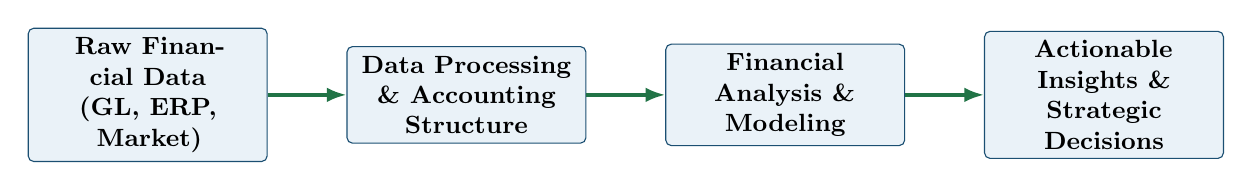
\begin{tikzpicture}[node distance=1.2cm, auto,
  block/.style={rectangle, draw=keyblue, fill=keybluelight, text width=2.8cm, text centered, rounded corners=2pt, minimum height=1cm, font=\small\bfseries},
  line/.style={draw=excelgreen, -{Latex[length=2.5mm]}, line width=1.2pt}]
  
  \node [block] (data) {Raw Financial Data \\ (GL, ERP, Market)};
  \node [block, right=1cm of data] (proc) {Data Processing \& Accounting Structure};
  \node [block, right=1cm of proc] (anal) {Financial Analysis \& Modeling};
  \node [block, right=1cm of anal] (dec) {Actionable Insights \& Strategic Decisions};
  
  \path [line] (data) -- (proc);
  \path [line] (proc) -- (anal);
  \path [line] (anal) -- (dec);
\end{tikzpicture}
\caption{The Financial Analytics Value Chain}
\label{fig:value-chain}
\end{figure}

\subsection{Core Importance of Financial Analytics}

\begin{itemize}
  \item \textbf{Understanding Business Performance:} Tracking historical and trailing revenues, cost structures, and gross/operating margins to pinpoint exact drivers of profitability and unit economics.
  \item \textbf{Risk Management \& Liquidity Control:} Identifying emerging financial vulnerabilities---such as working capital crunches, credit defaults, interest rate exposure, and foreign exchange risks---before they escalate into insolvency.
  \item \textbf{Strategic Growth \& Capital Budgeting:} Utilizing empirical historical trends and statistical regression to evaluate capital expenditure (CapEx), merger \& acquisition (M\&A) targets, and expansion into new markets.
  \item \textbf{Operational Efficiency \& Continuous Improvement:} Isolating variances between budgeted vs.\ actual performance ($BvA$) and diagnosing cost overruns across operational units.
  \item \textbf{Investor \& Stakeholder Confidence:} Delivering rigorous, GAAP/IFRS-compliant financial models and transparent reporting that foster trust among equity investors, lenders, rating agencies, and board members.
\end{itemize}

\begin{keyconcept}[The Core Mandate of the Financial Analyst]
A financial analyst does not simply document what happened in the past; they decode \textbf{why} it happened and quantify \textbf{what will happen next} under varying operational scenarios and capital market conditions.
\end{keyconcept}

\subsection{Tools of the Modern Financial Stack}

While modern data teams utilize diverse technical stacks, specialized financial analysis balances agility, formula transparency, and mathematical rigor:

\begin{table}[htbp]
\centering
\small
\begin{tabular}{L{3.2cm} L{3.5cm} L{7.5cm}}
\toprule
\textbf{Tool} & \textbf{Primary Domain} & \textbf{Role in Corporate Finance \& Analytics} \\
\midrule
\textbf{Microsoft Excel} & Financial Modeling & Ubiquitous standard for dynamic 3-statement models, DCF, LBO, valuation schedules, and board decks. \\
\textbf{Python} & Quant \& Automation & Large-scale time-series processing, Monte Carlo simulations, algorithmic risk models, and automated reporting. \\
\textbf{SQL} & Data Warehousing & Querying transaction ledgers, customer lifetime value (LTV) records, and multi-gigabyte ERP data pools. \\
\textbf{Power BI / Tableau} & Visual Dashboards & Executive KPI monitoring, interactive divisional reporting, and automated departmental scorecards. \\
\bottomrule
\end{tabular}
\caption{Modern Financial Analytics Technology Stack}
\label{tab:tech-stack}
\end{table}

\begin{financeapp}[Excel as the Primary Modeling Engine]
Despite advancements in Business Intelligence (BI) and quantitative programming languages, \textbf{MS Excel remains the primary language of global finance}. Its cell-level auditability, instantaneous scenario switching, and universal acceptance across Wall Street and corporate boards make it an indispensable tool for analysts.
\end{financeapp}

% ============================================================
\section{Master Tool: MS Excel (Foundations to Professional Modeling)}
\label{sec:excel-mastery}
% ============================================================

Excel is the foundational modeling environment across investment banking, private equity, corporate FP\&A, and equity research.

\subsection{Why MS Excel Dominates Financial Analysis}

\begin{enumerate}
  \item \textbf{Formula Powerhouse:} Access to hundreds of financial (\texttt{XNPV}, \texttt{XIRR}, \texttt{PMT}, \texttt{EFFECT}), logical (\texttt{IFS}, \texttt{SWITCH}, \texttt{LAMBDA}), and lookup functions (\texttt{XLOOKUP}, \texttt{INDEX-MATCH}) designed specifically for multi-variable economic modeling.
  \item \textbf{Dynamic Scenario Architecture:} Built-in sensitivity features such as Data Tables (1D and 2D), Goal Seek, and Scenario Manager allow instant valuation under Bull, Base, and Bear cases.
  \item \textbf{Data Integrity \& Validation:} Rules-based input controls, dynamic dropdown lists, and custom number formatting prevent circular logic, formatting errors, and broken formula linkages.
  \item \textbf{Auditability \& Cell Transparency:} Every intermediary step in a valuation or debt amortization schedule can be inspected, audited, and traced across precedents and dependents.
\end{enumerate}

\begin{protip}[Keyboard-First Workflow]
Professional financial modelers minimize mouse usage. Relying on keyboard shortcuts (\key{F4} for absolute referencing, \key{Alt + =} for AutoSum, \key{Alt + E + S + V} for Paste Special Values) boosts modeling speed by 300--400\%.
\end{protip}

% ============================================================
\section{Basic Accounting \& Financial Statements}
\label{sec:accounting-statements}
% ============================================================

Accounting is the formal language of commerce. Financial models are only as robust as the underlying accounting mechanics that govern them.

\subsection{The Fundamental Accounting Equation}

All corporate financial reporting is rooted in double-entry bookkeeping governed by the foundational balance equation:

\begin{formulabox}[The Fundamental Balance Sheet Equation]
\begin{align}
\text{Assets} &= \text{Liabilities} + \text{Shareholders' Equity} \\[4pt]
\text{Assets} &= \text{Liabilities} + \text{Contributed Capital} + \text{Beg. Retained Earnings} \nonumber \\
              &\quad + \text{Net Income} - \text{Dividends}
\end{align}
\end{formulabox}

\subsection{The Three Core Financial Statements}

\begin{figure}[htbp]
\centering
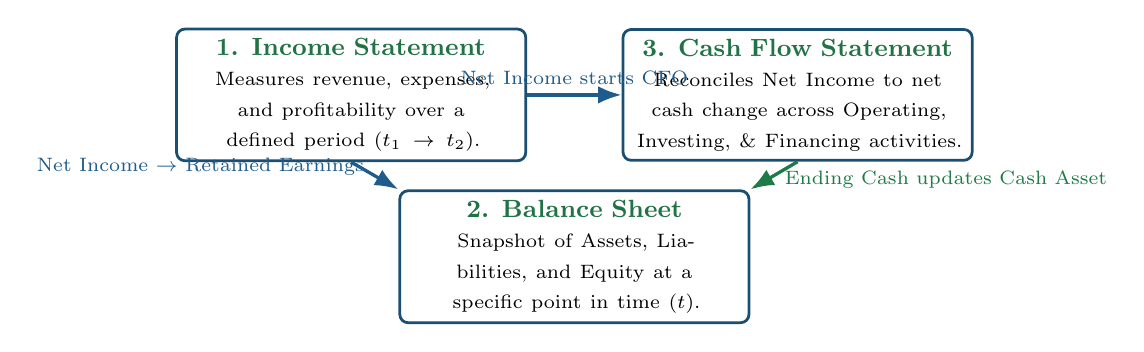
\begin{tikzpicture}[node distance=1.8cm, auto,
  box/.style={rectangle, draw=keyblue, fill=white, line width=1pt, text width=4.2cm, text centered, rounded corners=3pt, minimum height=1.6cm, font=\small},
  titlebox/.style={font=\bfseries\color{excelgreen}}]
  
  \node [box] (is) {\textbf{\color{excelgreen}1. Income Statement}\\ \scriptsize Measures revenue, expenses, and profitability over a defined period ($t_1 \to t_2$).};
  \node [box, right=1.2cm of is] (cfs) {\textbf{\color{excelgreen}3. Cash Flow Statement}\\ \scriptsize Reconciles Net Income to net cash change across Operating, Investing, \& Financing activities.};
  \node [box, below=1.2cm of $(is)!0.5!(cfs)$] (bs) {\textbf{\color{excelgreen}2. Balance Sheet}\\ \scriptsize Snapshot of Assets, Liabilities, and Equity at a specific point in time ($t$).};
  
  \draw [-{Latex[length=3mm]}, line width=1.2pt, pythonblue] (is.south) -- node[left, font=\scriptsize, align=right] {Net Income $\to$ Retained Earnings\\} (bs.north west);
  \draw [-{Latex[length=3mm]}, line width=1.2pt, pythonblue] (is.east) -- node[above, font=\scriptsize] {Net Income starts CFO} (cfs.west);
  \draw [-{Latex[length=3mm]}, line width=1.2pt, tipgreen] (cfs.south) -- node[right, font=\scriptsize, align=left] {\\Ending Cash updates Cash Asset} (bs.north east);
\end{tikzpicture}
\caption{The Dynamic Interlinkage of the Three Financial Statements}
\label{fig:3-statement-linkage}
\end{figure}

\subsubsection{1. Income Statement (Statement of Profit and Loss)}
Measures financial performance over a reporting duration (Quarter or Year).
\begin{itemize}
  \item \textbf{Revenue (Top Line):} Gross earnings generated from sales of goods or provision of services.
  \item \textbf{Cost of Goods Sold (COGS):} Direct variable costs directly attributable to the production of goods sold.
  \item \textbf{Gross Profit:} $\text{Revenue} - \text{COGS}$.
  \item \textbf{Operating Expenses (OpEx):} Selling, General, and Administrative (SG\&A), R\&D, and advertising costs.
  \item \textbf{Operating Income (EBIT):} Earnings Before Interest and Taxes ($\text{Gross Profit} - \text{OpEx}$).
  \item \textbf{Net Income (Bottom Line):} Profit remaining after deducting interest expense, non-operating items, and corporate income taxes.
\end{itemize}

\subsubsection{2. Balance Sheet}
A snapshot of what a company owns (Assets) and owes (Liabilities and Equity) at a single fiscal moment.
\begin{itemize}
  \item \textbf{Current Assets:} Cash, Short-Term Investments, Accounts Receivable (AR), and Inventory (liquid within 12 months).
  \item \textbf{Non-Current Assets:} Property, Plant, \& Equipment (PP\&E), Intangible Assets, Goodwill, and Long-Term Investments.
  \item \textbf{Current Liabilities:} Accounts Payable (AP), Accrued Expenses, and Current Portion of Long-Term Debt ($< 1$ year).
  \item \textbf{Long-Term Liabilities:} Senior Notes, Bonds Payable, Deferred Tax Liabilities, and Long-Term Lease Obligations.
  \item \textbf{Shareholders' Equity:} Common Stock, Additional Paid-In Capital (APIC), Retained Earnings, and Treasury Stock.
\end{itemize}

\subsubsection{3. Cash Flow Statement (CFS)}
Tracks actual liquidity moving in and out of the firm, categorized into three activities:
\begin{itemize}
  \item \textbf{Cash Flow from Operating Activities (CFO):} Begins with Net Income, adds back non-cash expenses (Depreciation \& Amortization), and adjusts for net changes in Working Capital ($\Delta\text{AR}, \Delta\text{Inv}, \Delta\text{AP}$).
  \item \textbf{Cash Flow from Investing Activities (CFI):} Capital expenditures (CapEx), acquisitions, and purchases/sales of marketable securities.
  \item \textbf{Cash Flow from Financing Activities (CFF):} Debt issuance/repayment, equity issuance, share repurchases, and dividend payouts.
\end{itemize}

% ============================================================
\section{Advanced Accounting Concepts \& Working Capital Management}
\label{sec:adv-accounting}
% ============================================================

\subsection{Revenue \& Cost Recognition Principles}

Accrual accounting decouples financial performance from cash timing:
\begin{itemize}
  \item \textbf{Revenue Recognition (ASC 606 / IFRS 15):} Revenue is recognized when performance obligations are satisfied (goods delivered or services rendered), regardless of when cash settlement occurs.
  \item \textbf{Matching Principle (Cost Recognition):} Expenses incurred to generate specific revenue must be recognized in the identical reporting period as the corresponding revenue.
\end{itemize}

\subsection{Working Capital Dynamics}

\textbf{Net Working Capital (NWC)} measures short-term operational liquidity:
\begin{equation}
\text{NWC} = \text{Current Assets (excl.\ Cash)} - \text{Current Liabilities (excl.\ Short-Term Debt)}
\end{equation}

\begin{table}[htbp]
\centering
\small
\begin{tabular}{L{3.5cm} L{3.5cm} L{7.5cm}}
\toprule
\textbf{Component} & \textbf{Key Metric} & \textbf{Operational Impact} \\
\midrule
\textbf{Trade Receivables} & \textbf{DSO} (Days Sales Outstanding) & $\frac{\text{Accounts Receivable}}{\text{Total Credit Sales}} \times 365$. Measures how quickly customers pay. Lower is better for cash velocity. \\
\textbf{Inventory Management} & \textbf{DIO} (Days Inventory Outstanding) & $\frac{\text{Ending Inventory}}{\text{COGS}} \times 365$. Quantifies average days inventory sits before being sold. Lower reduces holding cost. \\
\textbf{Trade Payables} & \textbf{DPO} (Days Payable Outstanding) & $\frac{\text{Accounts Payable}}{\text{COGS}} \times 365$. Average days company takes to pay suppliers. Higher preserves operational cash. \\
\bottomrule
\end{tabular}
\caption{Working Capital Performance Metrics}
\label{tab:wc-metrics}
\end{table}

\begin{formulabox}[Cash Conversion Cycle (CCC)]
The Cash Conversion Cycle represents the net elapsed time (in days) between purchasing raw inventory and collecting cash from customers:
\begin{equation}
\text{CCC} = \text{DIO} + \text{DSO} - \text{DPO}
\end{equation}
\end{formulabox}

\begin{keyconcept}[Negative Working Capital]
Firms with significant supplier bargaining power (e.g., Amazon, Apple) frequently operate with a \textbf{negative Cash Conversion Cycle} ($\text{DPO} > \text{DIO} + \text{DSO}$), effectively financing daily operations using vendor credit.
\end{keyconcept}

% ============================================================
\section{Business Analysis Techniques}
\label{sec:analysis-techniques}
% ============================================================

Financial professionals utilize quantitative frameworks to extract predictive insights from corporate data:

\begin{table}[htbp]
\centering
\small
\begin{tabular}{L{3.2cm} L{4.5cm} L{6.8cm}}
\toprule
\textbf{Analysis Type} & \textbf{Primary Focus \& Formula / Logic} & \textbf{Strategic Business Application} \\
\midrule
\textbf{Trend Analysis} & Tracking percentage change: $\frac{Y_t - Y_{t-1}}{Y_{t-1}}$ over historical multi-year series. & Detecting structural shifts in revenue growth, margin compression, or OpEx inflation. \\
\addlinespace
\textbf{Comparative Analysis} & Peer benchmarking against industry quartiles and sector averages. & Identifying competitive moat, pricing power, and cost disadvantages against rivals. \\
\addlinespace
\textbf{Regression Analysis} & Statistical modeling: $Y = \beta_0 + \beta_1 X_1 + \epsilon$. & Quantifying elasticity (e.g., impact of R\&D or marketing spend on incremental revenue). \\
\addlinespace
\textbf{Correlation Analysis} & Pearson coefficient: $r = \frac{\sum (x - \bar{x})(y - \bar{y})}{\sqrt{\sum(x-\bar{x})^2 \sum(y-\bar{y})^2}}$. & Evaluating portfolio co-movements, FX exposure, and commodity cost pass-through. \\
\addlinespace
\textbf{Time-Series Analysis} & ARIMA, exponential smoothing, and moving average seasonal decompositions. & Demand forecasting, inventory buffer planning, and cash flow liquidity stress-testing. \\
\addlinespace
\textbf{Value-Based Analysis} & $\text{EVA} = \text{NOPAT} - (\text{WACC} \times \text{Invested Capital})$. & Determining whether corporate capital allocation generates true economic profit above hurdle rates. \\
\bottomrule
\end{tabular}
\caption{Comprehensive Business Analysis Methodologies}
\label{tab:business-analysis}
\end{table}

% ============================================================
\section{The Time Value of Money (TVM)}
\label{sec:tvm}
% ============================================================

The foundational axiom of financial mathematics states:
\begin{center}
\large\bfseries\color{keyblue} ``A dollar received today is worth more than a dollar received in the future.''
\end{center}

\subsection{Underlying Catalysts of Time Preference}
\begin{enumerate}
  \item \textbf{Opportunity Cost of Capital:} Capital available today can be reinvested into productive assets or risk-free instruments to compound yield.
  \item \textbf{Purchasing Power Inflation:} Fiat currency typically loses purchasing power over time due to macroeconomic price inflation.
  \item \textbf{Credit \& Default Risk:} A future promise of payment carries inherent uncertainty, counterparty risk, and liquidity friction.
\end{enumerate}

\subsection{Core Mathematical Formulations}

\begin{formulabox}[Core TVM Formulas]
\begin{align}
\text{Future Value (FV):} \quad & FV = PV \cdot (1 + r)^n \\[6pt]
\text{Present Value (PV):} \quad & PV = \frac{FV}{(1 + r)^n} = FV \cdot (1 + r)^{-n} \\[6pt]
\text{Net Present Value (NPV):} \quad & NPV = \sum_{t=0}^{n} \frac{CF_t}{(1 + r)^t} \\[6pt]
\text{Perpetuity Present Value:} \quad & PV_{\text{perpetuity}} = \frac{C}{r} \quad (\text{Growing: } \frac{C_1}{r - g}) \\[6pt]
\text{Ordinary Annuity PV:} \quad & PV_{\text{annuity}} = C \cdot \left[ \frac{1 - (1 + r)^{-n}}{r} \right]
\end{align}
Where: $PV = \text{Present Value}$, $FV = \text{Future Value}$, $r = \text{Discount / Hurdle Rate per period}$, $n = \text{Number of compounding periods}$, $C = \text{Cash flow per period}$, $g = \text{Perpetual growth rate}$.
\end{formulabox}

\subsection{Comprehensive Worked Practice Problem}

\begin{workedexample}[Capital Budgeting Decision via TVM]
\textbf{Scenario:}\\
Acme Industrial Corp is evaluating the purchase of a new automated CNC machining line.
\begin{itemize}
  \item Initial Investment ($CF_0$): $\$250,000$ (outflow at $t=0$)
  \item Projected Net Annual Cash Inflows ($CF_1 \to CF_5$):
    \begin{itemize}
      \item Year 1: $\$60,000$
      \item Year 2: $\$75,000$
      \item Year 3: $\$85,000$
      \item Year 4: $\$90,000$
      \item Year 5: $\$70,000$
    \end{itemize}
  \item Weighted Average Cost of Capital ($\text{WACC} / r$): $10.0\%$ per annum.
\end{itemize}

\textbf{Task:}
\begin{enumerate}
  \item Calculate the discounted present value for each individual cash flow.
  \item Determine the project's Net Present Value ($NPV$).
  \item Advise corporate management on the capital investment decision.
\end{enumerate}

\tcbline
\textbf{Step-by-Step Solution:}

\vspace{0.2cm}
\begin{center}
\small
\begin{tabular}{C{1.2cm} R{2.3cm} C{2.3cm} R{2.3cm} R{2.6cm}}
\toprule
\textbf{Year ($t$)} & \textbf{Nominal Cash Flow} & \textbf{Discount Factor} $\frac{1}{(1.10)^t}$ & \textbf{Discounted PV} & \textbf{Cumulative PV} \\
\midrule
$0$ & $-\$250,000.00$ & $1.00000$ & $-\$250,000.00$ & $-\$250,000.00$ \\
$1$ & $\$60,000.00$ & $0.90909$ & $\$54,545.45$ & $-\$195,454.55$ \\
$2$ & $\$75,000.00$ & $0.82645$ & $\$61,983.47$ & $-\$133,471.07$ \\
$3$ & $\$85,000.00$ & $0.75131$ & $\$63,861.76$ & $-\$69,609.32$ \\
$4$ & $\$90,000.00$ & $0.68301$ & $\$61,471.21$ & $-\$8,138.11$ \\
$5$ & $\$70,000.00$ & $0.62092$ & $\$43,464.49$ & $\mathbf{+\$35,326.38}$ \\
\midrule
\multicolumn{3}{l}{\textbf{Total Present Value of Cash Inflows ($\sum PV_{1\to5}$):}} & \multicolumn{2}{r}{$\mathbf{\$285,326.38}$} \\
\multicolumn{3}{l}{\textbf{Net Present Value ($NPV = \text{PV Inflows} - \text{Initial Cost}$):}} & \multicolumn{2}{r}{$\mathbf{+\$35,326.38}$} \\
\bottomrule
\end{tabular}
\end{center}
\vspace{0.2cm}

\textbf{Excel Formula Implementation:}\\
\texttt{=NPV(10\%, 60000, 75000, 85000, 90000, 70000) - 250000} $\implies \mathbf{\$35,326.38}$

\textbf{Investment Recommendation:}\\
Because $\mathbf{NPV = +\$35,326.38 > 0}$ (and internal rate of return $\text{IRR} \approx 15.17\% > 10.0\%$), the project adds substantial economic value above Acme's hurdle rate. \textbf{Recommendation: Accept the investment.}
\end{workedexample}

% ============================================================
\section{Financial Modeling Architecture \& Best Practices}
\label{sec:modeling-architecture}
% ============================================================

Financial modeling is the discipline of constructing dynamic, mathematically integrated mathematical simulations of an enterprise's economic future.

\subsection{Primary Industry Model Archetypes}

\begin{enumerate}
  \item \textbf{Integrated 3-Statement Model:} The bedrock of corporate finance. Connects the Income Statement, Balance Sheet, and Cash Flow Statement dynamically via working capital, fixed asset depreciation schedules, and debt revolvers.
  \item \textbf{Discounted Cash Flow (DCF) Model:} Determines the intrinsic enterprise and equity value of a firm based on the net present value of its future Unlevered Free Cash Flows ($\text{UFCF}$):
  \begin{equation}
  \text{UFCF} = \text{EBIT} \times (1 - t) + \text{D\&A} - \text{CapEx} - \Delta\text{NWC}
  \end{equation}
  Terminal value is capitalized using either the Gordon Growth model ($\frac{\text{UFCF}_{N+1}}{\text{WACC} - g}$) or Exit Multiples ($\text{EV/EBITDA} \times \text{EBITDA}_N$).
  \item \textbf{Comparable Company Analysis (Trading Comps / CCA):} Relative valuation technique that benchmarks the target firm against publicly traded peers using market multiples ($\text{EV/EBITDA}$, $\text{P/E}$, $\text{EV/Sales}$, $\text{P/B}$).
  \item \textbf{Precedent Transactions Analysis:} Valuing a company based on multiples paid in past M\&A transactions within the same sector (includes control premiums).
  \item \textbf{Leveraged Buyout (LBO) Model:} Analyzes the feasibility of acquiring a firm using a high proportion of debt, modeling returns via Internal Rate of Return (IRR) and Multiple on Invested Capital (MoIC).
\end{enumerate}

\subsection{Institutional Modeling Standards \& FAST Conventions}

To maintain auditability across large deal teams, institutional models follow standard color-coding and layout rules:

\begin{table}[htbp]
\centering
\small
\begin{tabular}{L{3.2cm} L{3.5cm} L{7.5cm}}
\toprule
\textbf{Convention} & \textbf{Visual Style} & \textbf{Rule Description} \\
\midrule
\textbf{Hardcoded Inputs} & \textcolor{blue}{\textbf{Blue Font}} (RGB: 0, 0, 255) & Every historical value, inflation rate, revenue growth assumption, and tax rate input. \\
\addlinespace
\textbf{Formulas \& Math} & \textbf{Black Font} (RGB: 0, 0, 0) & Calculations, subtotals, and logic referencing other cells on the active sheet. \\
\addlinespace
\textbf{Inter-Sheet Links} & \textcolor{tipgreen}{\textbf{Green Font}} (RGB: 0, 128, 0) & References pulling data from different worksheets or companion modules. \\
\addlinespace
\textbf{External Data} & \textcolor{warnred}{\textbf{Red Font}} (RGB: 255, 0, 0) & Live feeds, Bloomberg/FactSet/CapIQ API formulas, or data requiring auditing. \\
\bottomrule
\end{tabular}
\caption{Institutional Financial Modeling Color Conventions}
\label{tab:color-conventions}
\end{table}

\begin{pitfall}[Never Hardcode in Formulas]
Avoid mixing assumptions directly into formulas (e.g., writing \texttt{=C14*1.05} instead of \texttt{=C14*(1+\$B\$4)}). Hardcoded constants inside calculation formulas create severe auditing blind spots and broken dependencies.
\end{pitfall}

\section{Summary \& Next Steps in the Handbook}

\begin{itemize}
  \item Proceed to \textbf{Module 1: Excel Foundations} for hands-on drills on data types, cell formatting, mathematical and text functions, and shortcut workflows.
  \item Continue to \textbf{Module 2: Making Excel Professional} to master dynamic referencing, macros, data validation, and model optimization.
  \item Complete \textbf{Module 3: Advanced Financial Modeling} to build full 3-statement forecast models, DCF valuation waterfalls, and sensitivity tables.
\end{itemize}

\end{document}
